\documentclass{article}
\usepackage{hyperref}
\usepackage{graphicx}
\usepackage{float}
\begin{document}
\title{Sensors for FRC}

\author{SoftwareBug2.0, Team 1425}
\date{\today}

\maketitle

\tableofcontents

\section{Introduction}

In designing a robot it's critical to pick out the right sensors.  There is a large variety of available sensors, there's more a problem of We'll go through a variety of types.  This document will attempt to give some idea of how different types of sensors work, when different types of sensors might be useful and what the trade-offs of using them are.  

%for each type:
%theory of operation
%output results \& accuracy/what it measures
%example use
%selection criteria \& different types
%programming schemes
%reliability
%	-failure modes
%		-environmental
%		-detectability
%		-non-environmental
%wiring
%cost, availablity
%power use
%weight
%types known to be used on FIRST robots

\section{Limit switches and bump sensors}

\begin{figure}[ht]
\centering
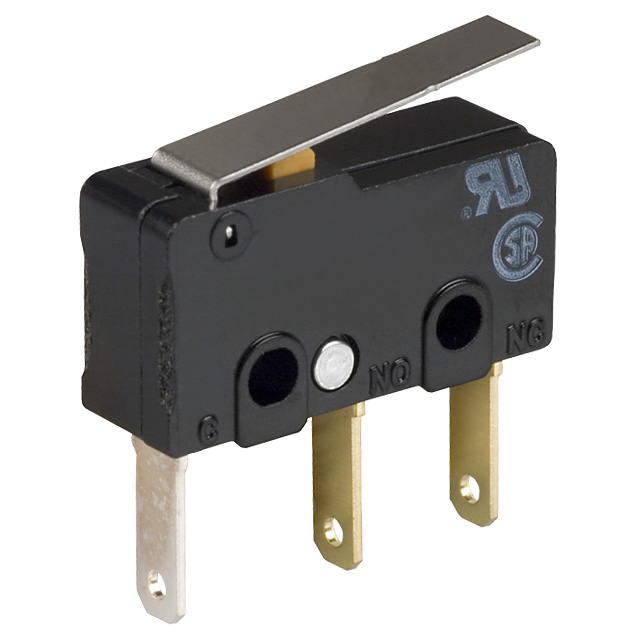
\includegraphics[width=2in]{Spdt_limit_switch.jpg}
\caption{Typical limit switch}
\end{figure}

\begin{figure}[ht]
\centering
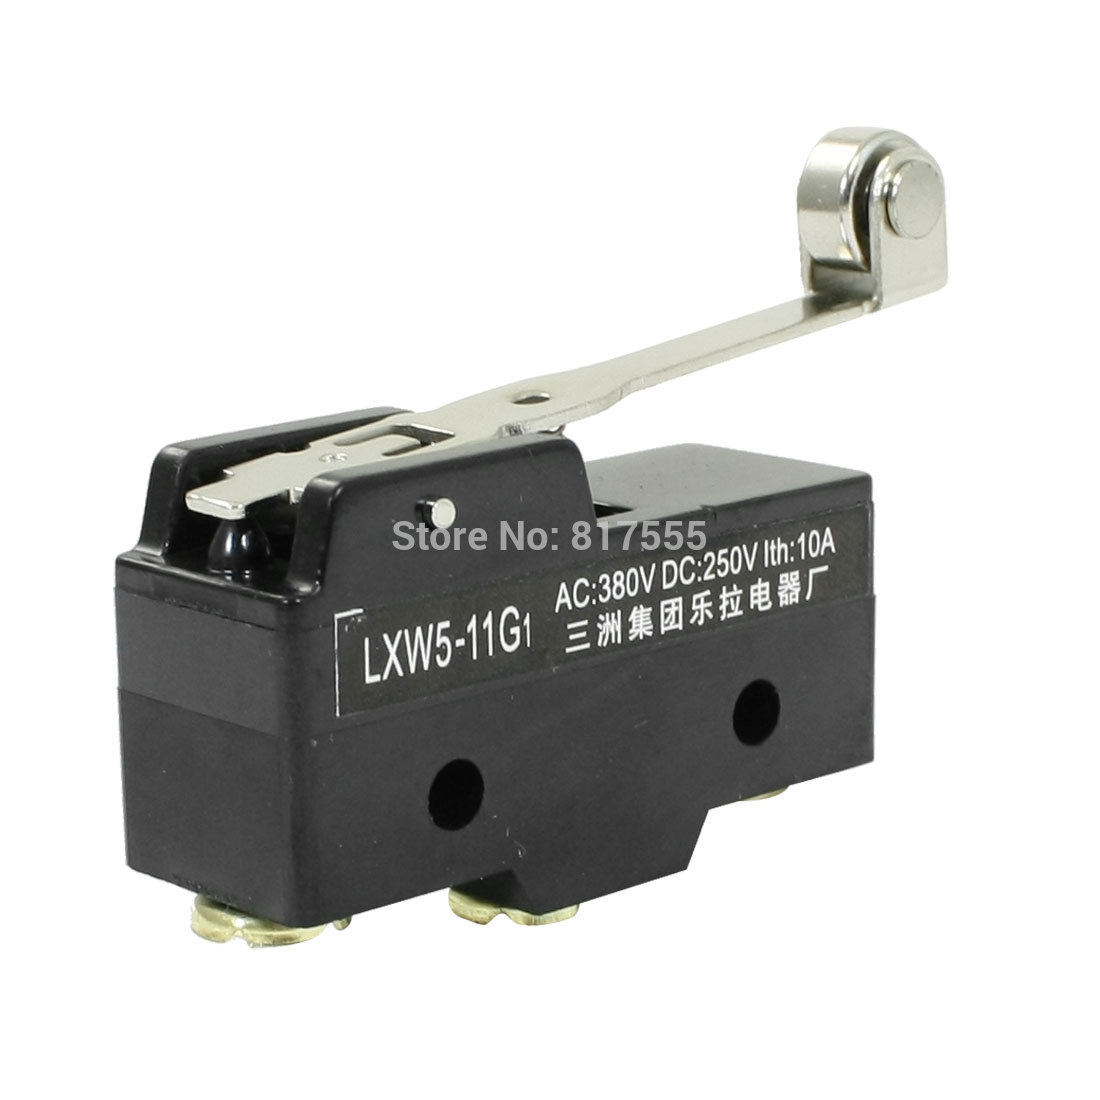
\includegraphics[width=2in]{limit_wheel.jpg}
\caption{Limit switch with roller}
\end{figure}

\begin{figure}[ht]
\centering
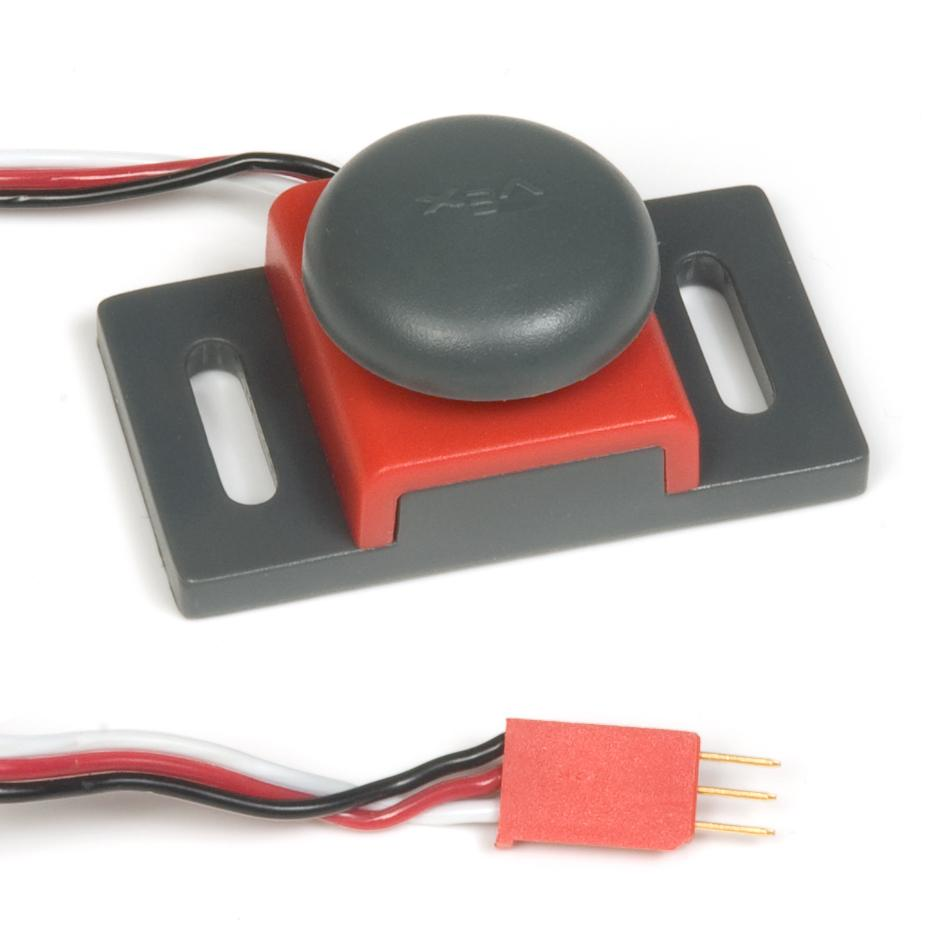
\includegraphics[width=2in]{vex_switch.jpg}
\caption{Vex-brand bump sensor}
\end{figure}

Limit switches and bumb sensors work by physically opening and closing a connection between two sets of contacts.  They produce a binary output and tend to have good repeatability of when they change states.  We used some of these on our 2004 robot to stop an arm extension when it was at either end.  

The major differentiating factor between these switches is their physical package.  Pick the one that can be mounted well and is least likely to become physically broken in a given application.  

These would typically be wired to a digital IO with an extra resistor soldered somewhere.  These types of switches are widely available (always in stock at Fry's) and many switches of this types are not more than a couple dollars.  When properly wired they should have negligible energy use and should weigh under an ounce.  

\section{Encoders}

\begin{figure}[ht]
\centering
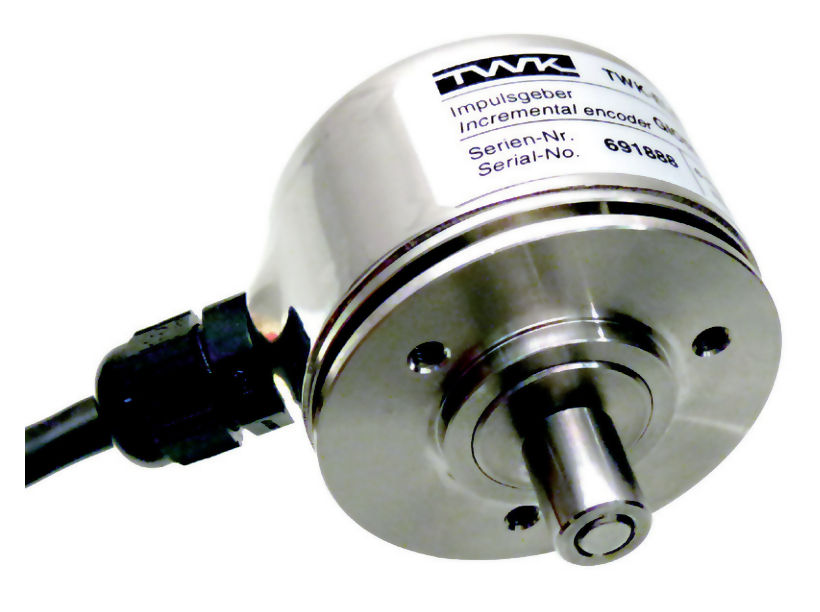
\includegraphics[width=2in]{encoder_shaft.jpg}
\caption{Encoder with integrated shaft}
\end{figure}

\begin{figure}[ht]
\centering
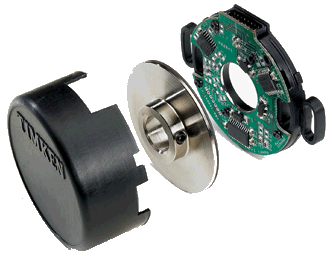
\includegraphics[width=2in]{encoder_slip.png}
\caption{Enc1oder which slips onto a shaft}
\end{figure}

Encoders are used to measure rotation.  They produce electrical pulses at some fixed interval of rotation so counting the number of pulses allows knowing how much rotation there was.  Internally this may be accomplished either optimcally or magnetically.  

We've used encoders on our drive wheels to be able to tell how far we've driven and also on our 2015 robot's elevators to keep track of how high we are.  These are one of the most common types of sensors on FRC robots.

Some encoders only count how much travel there has been while others have the ability to tell the direction of movement.  These are called quatrature encoders.  Encoders are available with a variety of resolutions.  For example, a 360-count encoder will have one pulse every time the shaft turns one degree.  Higher-count encoders give more precise answers but also require that the system reading them be able to read its inputs faster.  

Encoders may be wired to digital IO ports on the roboRIO or to a port on a Talon SRX.  When properly used encoders are very reliable.  We have a history of improper use.  

Costs of encoders vary but can be in the \$40 range.  Local sources are not likely, or at least not likely to have exactly the right type.  Power usage is negligible.  Weights can vary betwwen one ounce and 6 ounces.  

\section{Hall-effect sensors}

\begin{figure}[ht]
\centering
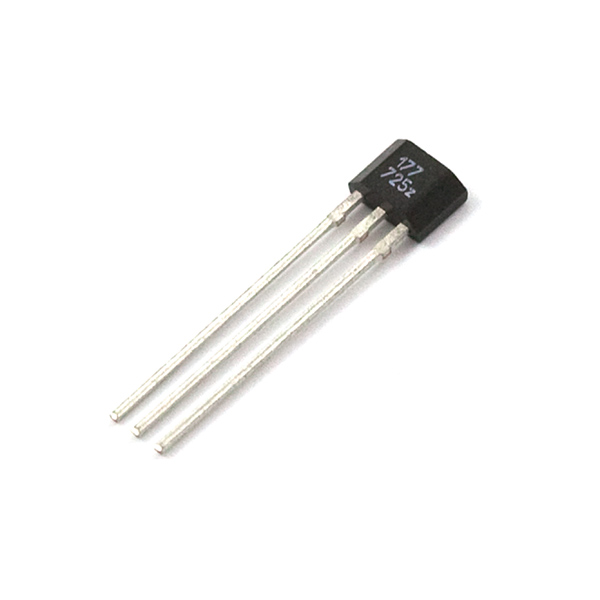
\includegraphics[width=2in]{hall_effect.jpg}
\caption{Basic Hall-effect sensor}
\end{figure}

\begin{figure}[ht]
\centering
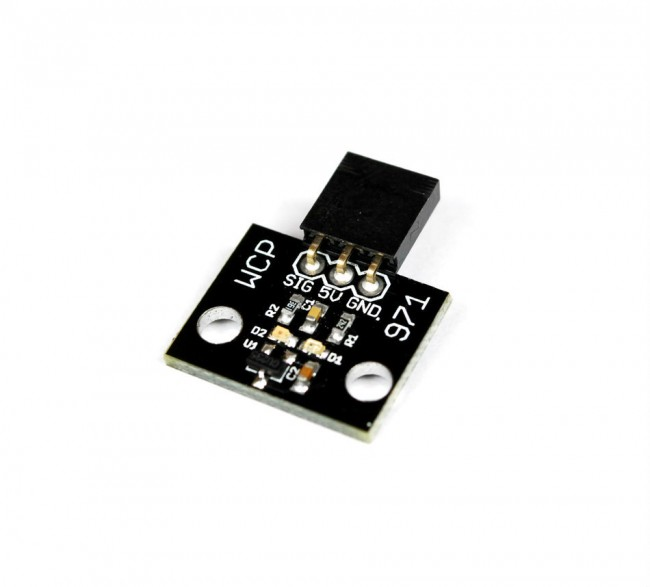
\includegraphics[width=2in]{hall-effect-sensor-board.jpg}
\caption{Pre-made Hall-effect sensor board}
\end{figure}

Hall effect sensors detect magnets.  They are often used like a limit switch, in which case they can be used to measure proximity rather than direct touching.  They can also be used in place of an encoder in high-speed applications where a very low number of counts per revolution is desirable.  

We have used these to measure speeds on shooters on several robots.  We also used one to measure when an actuator had reached its end on our 2014 robot.  

These produce a digital output and are approximately as reliable as the mounting system.  These are programmed the same as a limit switch.  Wiring wise, these can be bought as a bare sensor in which case some circuitry is required to be made, or as a complete setup.  The sensor itself is approximately \$1, while a pre-made board is approximately \$10.  In either case they should weigh under 1/4 of an ounce.  

\section{Magnetic pneumatic cylinder sensor}
\begin{figure}[ht]
\centering
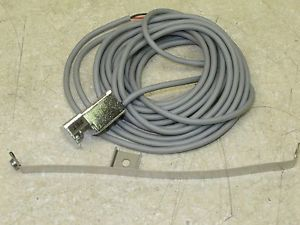
\includegraphics[width=2in]{cylinder_switch.JPG}
\caption{Bimba-brand switch with mounting hardware}
\end{figure}

These clamp on to the side of a pneumatic cylinder and reads when the end of the piston is near.  This relies on using a type of pneumatic cylinder that has a magnet inside.  When used in conjunction with the proper type of pneumatic solenoid this allows repeatably stopping a cylinder at a location part way through its stroke.  

We used these on our 2013 robot for raising and lowering our shot.  For programming it's important to look for the edges of when the sensor turns on or off, and note that coming from different directions will yield different results.  

I have never seen one of these fail.  Wiring is directly into a digital IO.  Cost is about \$15 and we should already have some in stock.  Power usage is negligible.  Weight should not be more than a couple of ounces.  

\section{Potentiometers}
\begin{figure}[ht]
\centering
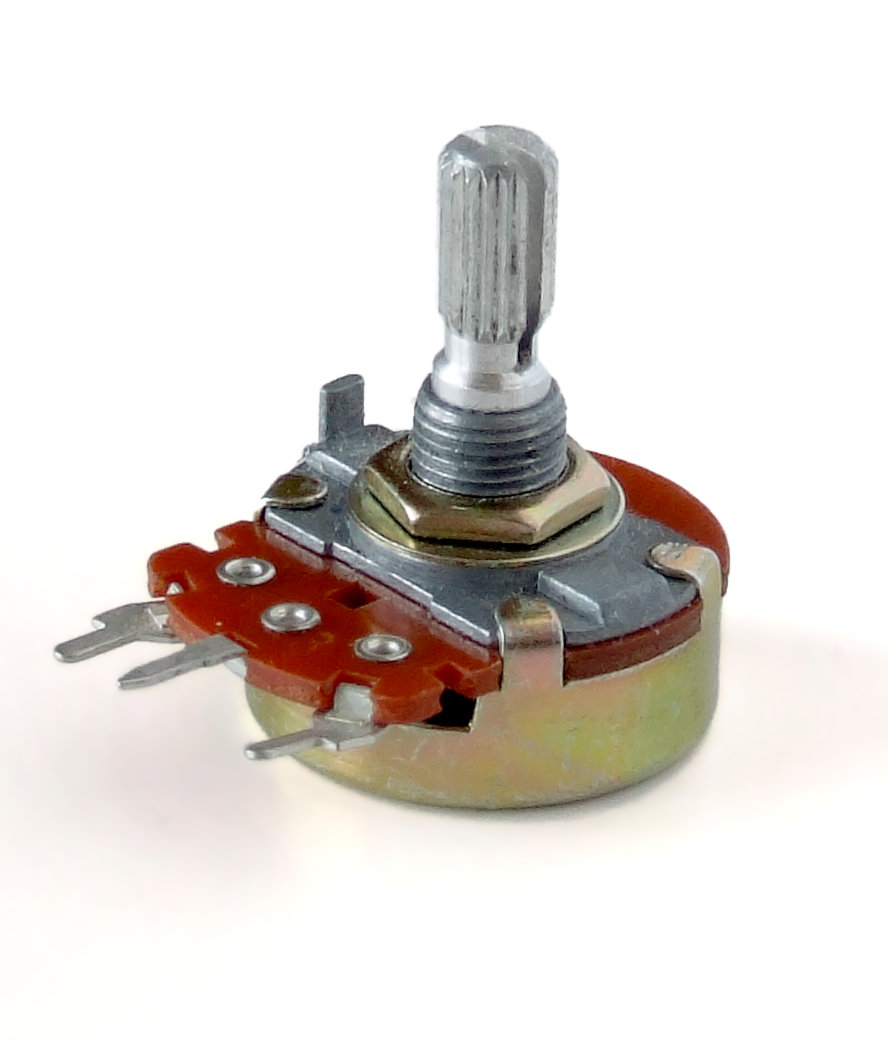
\includegraphics[width=2in]{Potentiometer.jpg}
\caption{Potentiometer.  The shaft that extends vertically rotates.}
\end{figure}

Potentiometers are a resistor which changes resistence as an input is moved.  Commonly, it might go from approximately 0 Ohms to 5k Ohms.  This is used to produce a variable voltage which can be directly mapped to a particular angle of the shaft.  

We used a potentiometer to tell us the angle of our collector on our 2016 robot.

These are not typically considered high-precision.  A shaft potentiometer might have a range of motion of 270$^{\circ}$ but it could also happen in two complete revolutions, in which case it would be called a 2-turn pot.  Slide-potentiometers are also available, which change their outputs based on a linear motion.

Potentiometers can be broken by being turned beyond their intended range.  This may be detectable if its output stops changing when it ought to.  Frys typically will have potentiometers in stock for \$10-\$20.  A typical weight would be about .7 ounces.  

\section{Current sensing}
\begin{figure}[ht]
\centering
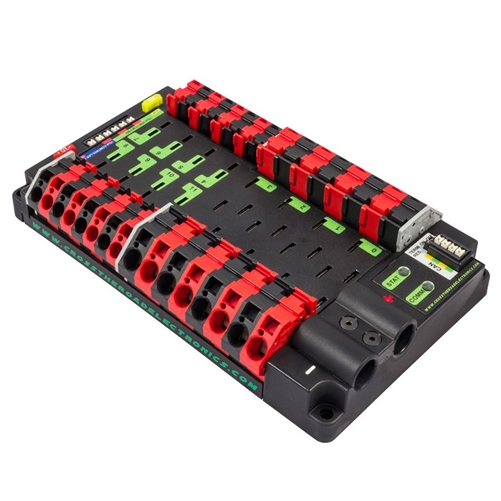
\includegraphics[width=2in]{pdp.jpg}
\caption{The power distribution panel contains built-in current sensing for each output.}
\end{figure}

The amount of electrical power used to drive different outputs may tell something about the state of the device.  For example, if a motor is told to turn but no current is drawn then something has gone wrong with the system.  Typically current is measured in amps.  
We used current sensing on our 2016 robot to let us know when the drivebase had hit a wall during autonomous mode.  It's also possible to use current use to regulate the amount of force applied by an actuator.  

A variety of current sensors are available, however the easiest thing is to use the built-in current sensing capability of the PDP.  We have not run any experiments about the accuracy or precision of the PDP's current sensing, however it has been sufficient for everything that we've attempted to do with it.  

\section{Microphones}
Microphones are not typically used in FRC because for two reasons: 1) there is not typically anything for the robot to listed for, and 2) the environment is noisy, making it hard to distinguish different sounds.  

\section{Ultrasonic}
\begin{figure}[ht]
\centering
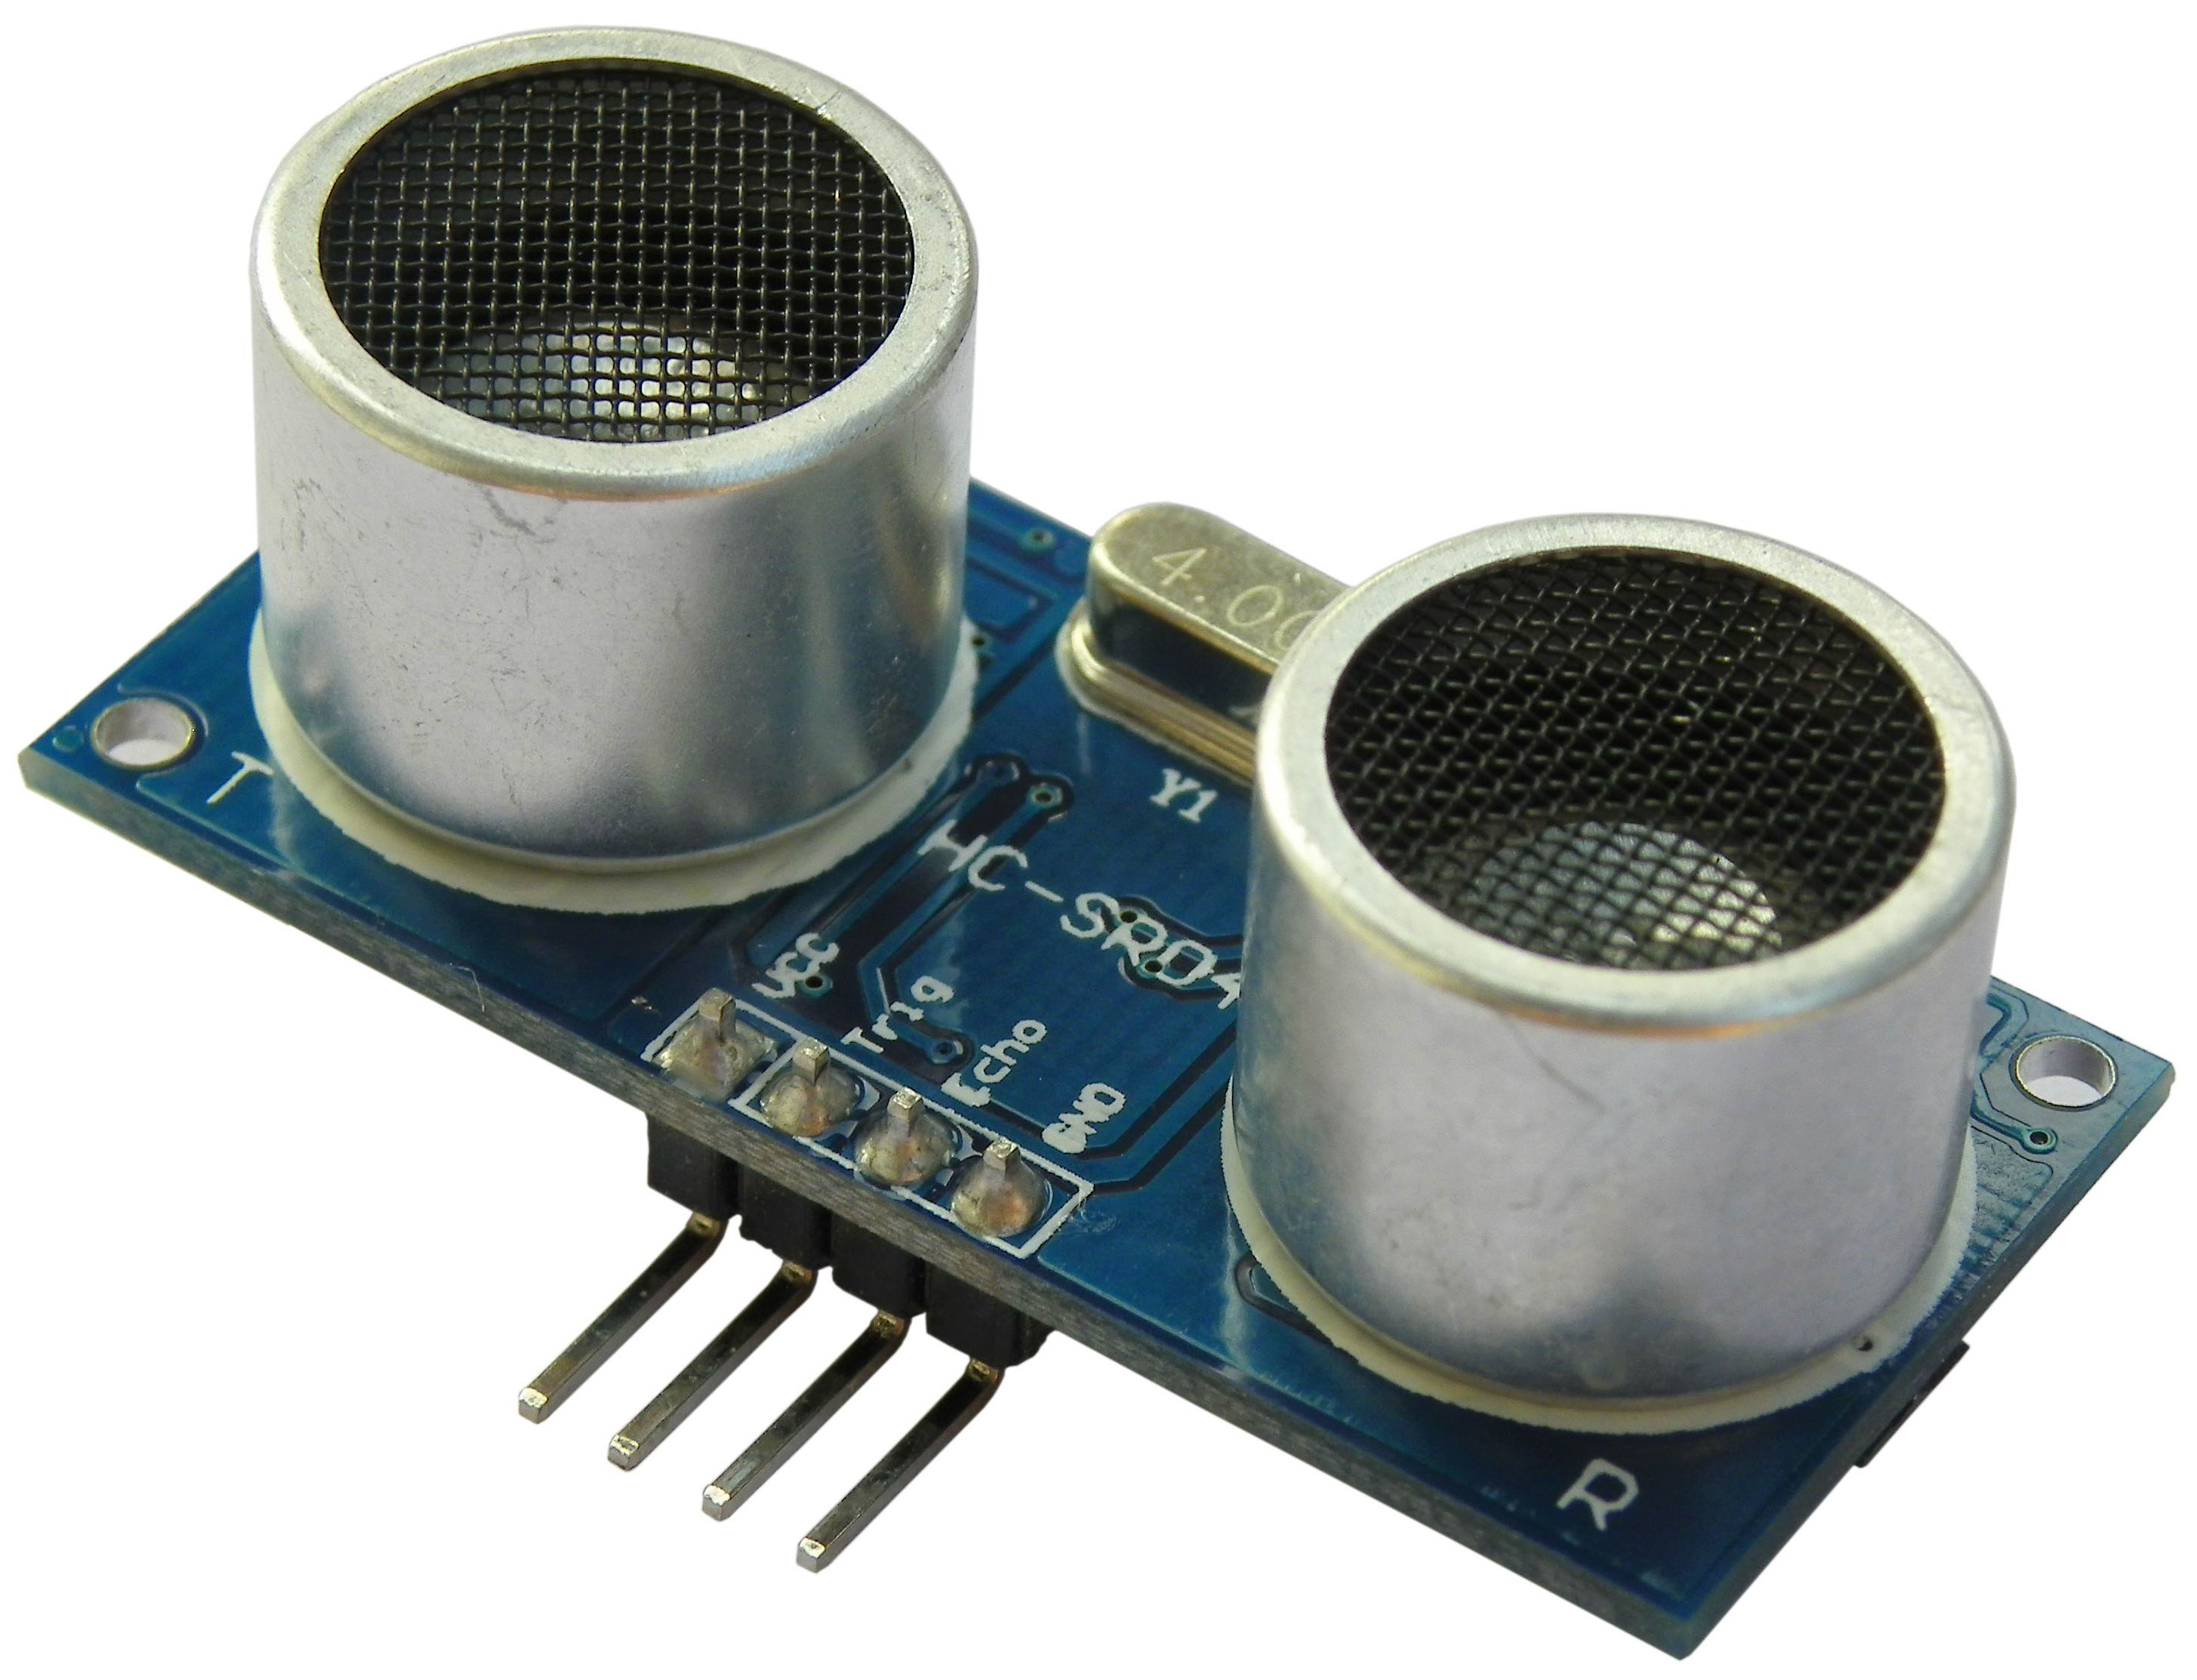
\includegraphics[width=2in]{HC-SR04-lg.jpg}
\caption{HC-SR04 ultrasonic sensor}
\end{figure}

\begin{figure}[ht]
\centering
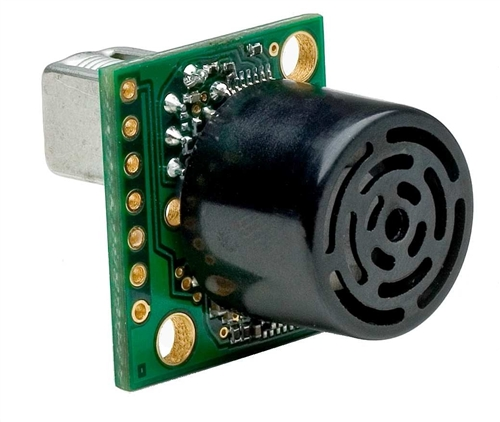
\includegraphics[width=2in]{ultrasonic.jpg}
\caption{An ultrasonic sensor available from AndyMark}
\end{figure}

Ultrasonic sensors measuring distance by sending out noises and then measuring their return from the environment.  These are typically only useful at short range (inches) and not especially precise.  

These are often used on small robots to avoid hitting walls.  

We have not used these in competition for some time.  However, we used an array of them on our 2007 robot in order to line up in autonomous mode on a target that would move from round to round.  At the 2016 PNW District Championship we talked to several teams who had and they were univerally underwhelmed.  It's not clear if this is because the sensors the teams have been experimenting with are of poor quality or if they've simply been unable to apply them correctly.

\section{Compass}

Compass sensors are exactly what they sound like: A compass with an electronic readout.  They work by measuring magnetic fields.  They are readily available and some teams have used them.  However, competitions are likely to be held in buildings made out of steel-reinforced concrete, and among a bunch of electromagnets, interfering with the detection of earth's magnetic field rendering compass sensors unreliable.

\section{Accelerometers}
\begin{figure}[ht]
\centering
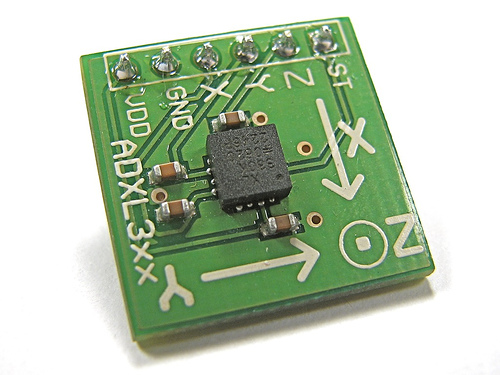
\includegraphics[width=2in]{accelerometer.jpg}
\caption{A breakout board with axes labeled.  The black chip in the center is the accelerometer itself.}
\end{figure}

\begin{figure}[ht]
\centering
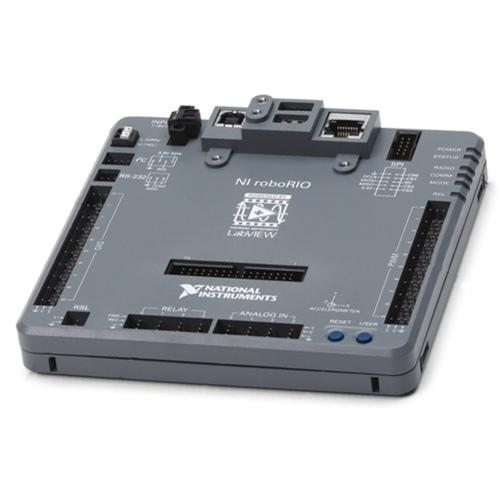
\includegraphics[width=2in]{roborio.jpg}
\caption{The roboRIO contains a built-in three-axis accelerometer.}
\end{figure}

Accelerometers measure the net force exerted upon them.  Most commonly, this force is the force of the mount holding the sensor up.  For this reason, they can be used as tilt sensors.  With a little more processing they can be used to approximate velocity and location.  

Accelerometers used in FRC are typically of the 3-axis type, where there is a measurement in each of the X, Y, and Z directions.  In fact, there is one of these built into the roboRIO.  We have not used it extensively.  A wide variety is commercially available, from \$10 to above the FRC price limit.  

In theory the math to calculate velocity and position from an accelerometer is easy, though perhaps a bit obscure to someone who hasn't taked calculus yet.  In practice care must be taken to keep small errors from compounding enough to produce results that quickly become worthless.  The tendency for accelerometers to produce results that gradually diverge from reality is called drift.  

\section{Gyros}
Gyros are not just a delicious sort of greek food.  They measure rotation of themselves in space.  They can be used to help robots drive straight, as with our 2013 robot, or to keep track of a heading in order to allow field-relative control, or in conjuntion with accelerometers to keep track of where are robot is on the field.  

Gyros typically come in 1-axis and 3-axis varieties.  Prices and availability vary widely but don't count on any particular one to be available locally.  

\section{IMU}
\begin{figure}[ht]
\centering
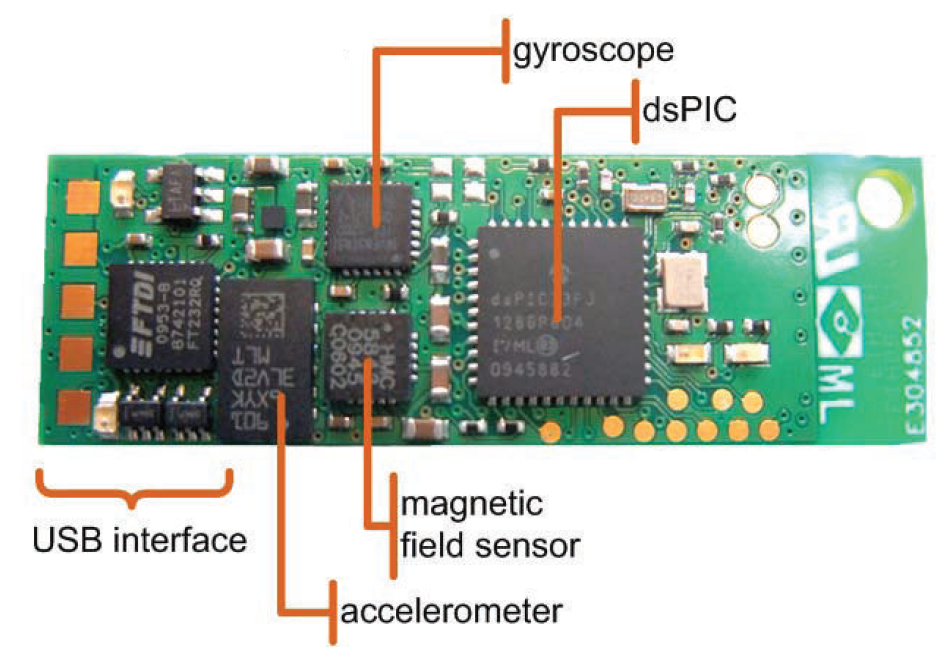
\includegraphics[width=2in]{imu.png}
\caption{An IMU, with parts labeled}
\end{figure}

Inertial measurement units combine accelerometers, gyros, and sometimes compasses in a single package.  A wide variety is available: some are relatively inexpensive, while others far exceed the FRC cost rules.  We have a pairs of ones that we got in FIRST Choice which would normally be well above the price limit.  We have not successfully used them yet, however.  On professional-grade mobile robots this is one of the most important parts of the whole machine.  

\section{GPS}
GPS is not used on FRC robots for two reasons: 1) events are held indoors and the reception would be terrible and 2) doing so would violate the rules about devices that send and receive signals.  GPS is typically the most reliable source of location data for robots that operate outdoors.  

\section{IR Sensor}
\begin{figure}[ht]
\centering
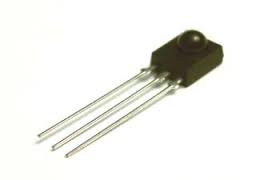
\includegraphics[width=2in]{ir_sensor.jpeg}
\caption{An IR sensor}
\end{figure}
IR sensors measure infrared light, which is not visible to the human eye but which is produced naturally with by the sun, by anything warm, and by electronic IR transmitters.  The most basic type produces an analog signal which varies with the intensity of the IR received.  These are not precision instruments.  

In 2004 the field had built-in IR beacons, which meant that teams could detect them in order to go to certain parts of the field.  

Wiring is straightforward, cost is minimal, power use is minimal, and weight is on par with a large LED.  

\section{Beam}
\begin{figure}[ht]
\centering
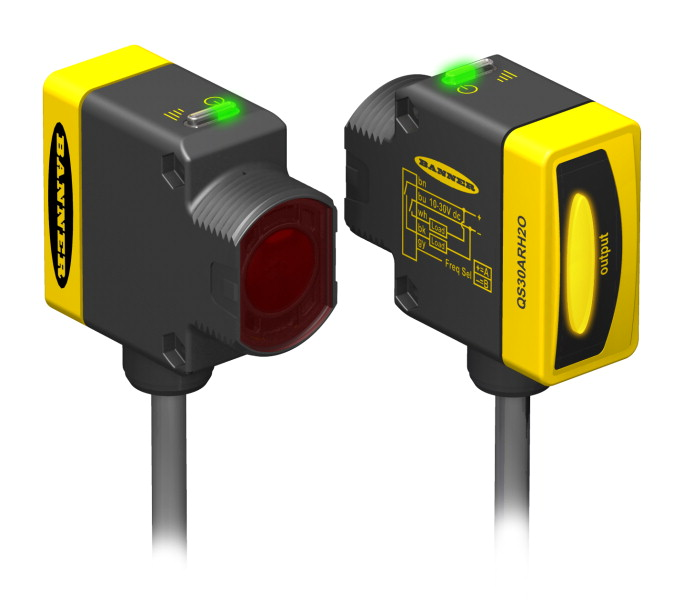
\includegraphics[width=2in]{beam.jpeg}
\caption{This Banner-brand beam sensor is designed for detecting the presence of fluids}
\end{figure}

A beam sensor consists of two parts: an emitter and a receiver.  The emitter outputs an IR beam and the receiver detects the presence or absense of that beam, which basically means whether or not something is in the way.  Large versions of these are usually on garage doors.

These are commonly used internally in robots to keep track of the locations of game pieces.  The most common failure is a misalignment between the transmitter and receiver.  These might cost around \$40.  

\section{IR rangefinder}
\begin{figure}[ht]
\centering
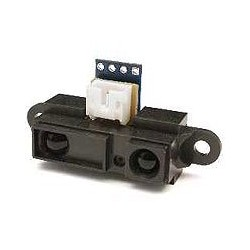
\includegraphics[width=2in]{ir-rangefinder.jpg}
\caption{Sharp-brand analog IR rangefinder}
\end{figure}

IR rangefinders emit IR and then measure the what angle it's reflected back in order to give a distance.  These are useful with a minimum distance of several inches and a maximum of several feet.  These are not high-precision devices but the same unit tends to be fairly repeatable when looking at the same surface.  

There are also digital versions that measure only the presence or absense of an object.  We successfully used the analog type on our Bunnybot for the pool-themed game and the digital kind on our 2015 robot to sense the presence of totes, and on our 2016 robot to measure the presence of balls that had been picked up.  

Wiring is simple and these run in the range of \$10-\$20.
\section{Light sensor}
\begin{figure}[ht]
\centering
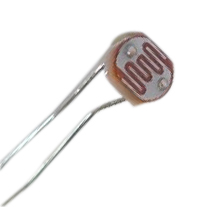
\includegraphics[width=2in]{light_sensor.jpg}
\caption{A bare light sensor}
\end{figure}

Light sensors measure the presence or absence of light.  They operate similarly to IR sensors.  

We successfully used a light sensor on our 2004 robot to detect lines on the floor during autonomous mode to help us know where different parts of the field were.  An important implementation detail that may improve the accurace of such systems is to add a skirt around the area with the sensor and your own light source in order to reduce dependency on the surrounding illumination.  

Light sensors are cheap and plentiful.

\section{Camera}

\begin{figure}[ht]
\centering
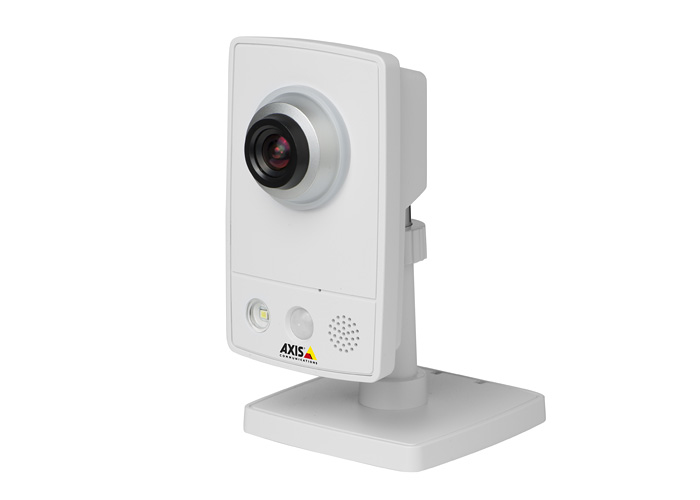
\includegraphics[width=2in]{M1034-W_axis_camera_large_2.jpg}
\caption{M1034-W Axis camera}
\end{figure}

Cameras on robots work in the same way as a camera in a cell phone.  They can be used in two different ways: to show images to a driver or to be used in machine vision.  

We've successfully sent images back to the drivers in 2012 to help with picking up balls, 2012 and 2014 to help with aiming and in 2016 to help lining up our climb.  We have a history of having computer vision systems that get close but are not actually used in play, such as 2012, 2014 and 2016.  We actually used a camera during play in 2006 although its utility was marginal at best.  

Cameras themselves tend to be fairly reliable, though we have broken them multiple times.  If images are sent back to the driver station this takes extra bandwidth, which may not always be available.  For example, we had a match replayed in 2012 and the reson ended up being that a majority of the robots on the field were using cameras and exhausting the medium.  This was discovered when the replay failed the same way as the original match.  The major risk with computer vision though is that the processing algorithms fail in unexpected ways when moving to a new environment.  For example, team 2471 could never get their image processing back to working properly at the 2016 championship event.  

There is a wide array of capability and expense in cameras.  Teams have been successful with nothing more than a USB webcam.  We've typically used ethernet-based cameras although we did use one with some integrated processing in 2006.  

Machine vision is well established in industrial settings and there are suppliers which sell modern integrated camera-processing systems such as Cognex.  Unfortunately, these tend to not fall within the allowed price range.  

Cameras and associated processing equipment have the potential to be power-hungry and also sensitive to power issues such as voltage drops and spikes.  

\subsection{Stereo imaging}
\begin{figure}[ht]
\centering
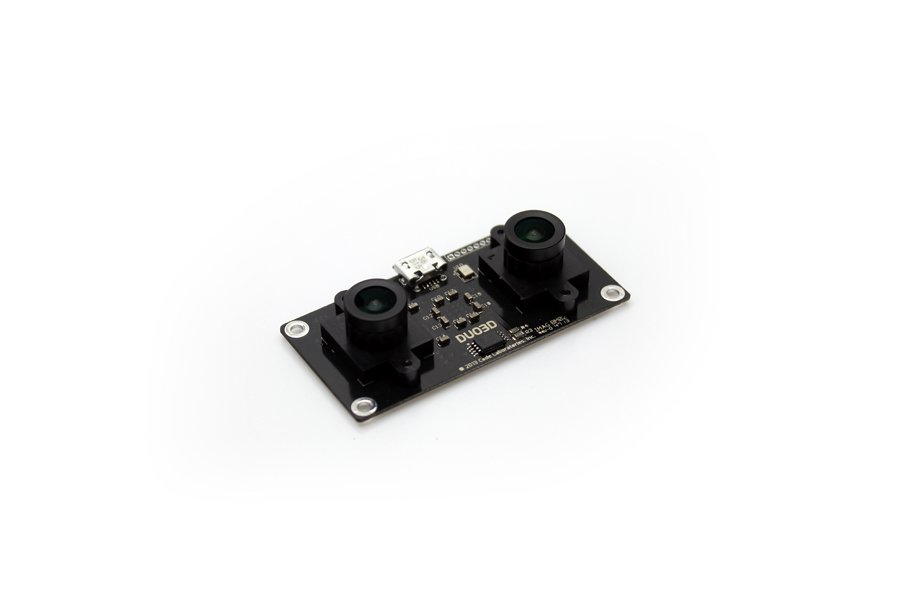
\includegraphics[width=2in]{stereo_camera.jpg}
\caption{DUO mini - USB Stereo Camera}
\end{figure}

Stereo imaging uses a pair of cameras pointed in the same direction in order to capture depth information.  I've heard of a team that sent stereo images back to the driver.  I haven't heard of any team that successfully did image processing based on stereo images.In some research circles stereo imaging has become infamous for the amount of effort required to get useful results.  

\subsection{Xbox Kinect}
\begin{figure}[ht]
\centering
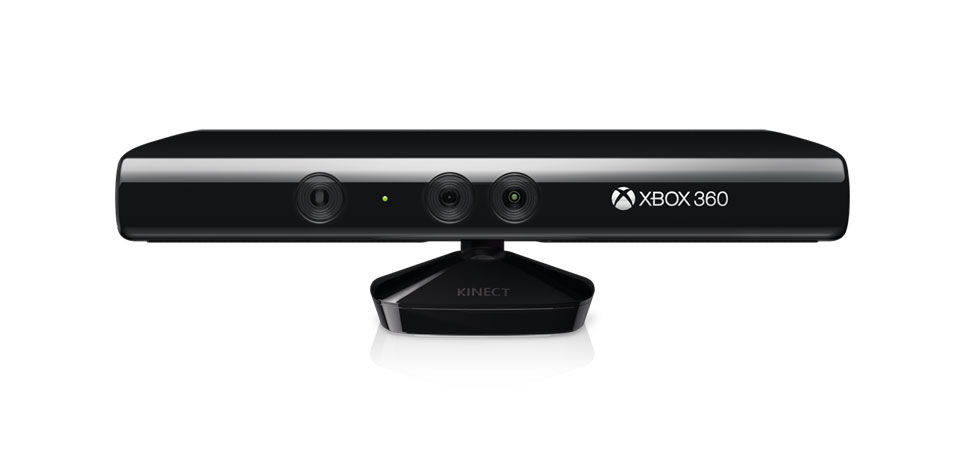
\includegraphics[width=2in]{kinect.jpg}
\caption{An Xbox Kinect}
\end{figure}
The Xbox Kinect creates an image with a distance assigned to each part of it.  It does this by projecting an IR grid onto the world and seeing what parts of the grid hit what parts of the picture.  This tends to be reliable except in the presense of a strong IR source such as the sun or stage lighting.  What this would mean for us is that we might look great at our first two events but then look terrible at the district championship or at worlds.

\section{Lidar}
\begin{figure}[ht]
\centering
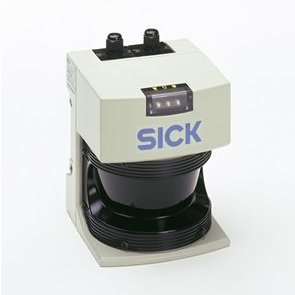
\includegraphics[width=2in]{SICK_LMS291.jpg}
\caption{A SICK LMS291 Lidar (circa 2004)}
\end{figure}

Lidar sends laser pulses in many directions so that the locations of objects can be inferred.  I don't know of any FRC team that has even attempted to use Lidar.  There are several reasons for this:
\begin{itemize}
\item There are FRC rules about lasers and most (and it used to be all) Lidar sensors run afoul of them.  
\item Most Lidar units exceed the cost limits.  Historically, the lowest-end models would still be in the thousands of dollars although costs have come down.  
\item A high level of programming effort is required.  
\end{itemize}

It might be looking into it from time to time as newer lower cost options become available.

\section{RADAR}
RADAR works by bouncing radio waves off of objects.  It is typically used at distances larger than those on an FRC field.  

\section{Conclusion}
Please direct any comments, questions or corrections to SoftwareBug2.0 on Chief Delphi.  

\end{document}
